\chapter{Dry sand mining}
%\section{River bank instability due to sand mining}
%Much like the Paraná Guazú, sand mining is a relevant topic in the lower Mekong river. Previous studies have shown that incision due to the sand mining exists in this river and is of the order of 0.13 m per year \autocite{brunierRecentMorphologicalChanges2014}. \citeauthor{hackneyRiverBankInstability2020} showed that this river bed lowering not only has morphological consequences but also geotechnical ones, since a lower river bed can cause instability of the river banks.

%In the previous study it was found that, even in conservative scenarios, entire sections of river banks along the lower Mekong River would shift from a stable to a seasonally unstable condition. This means they are likely to fail during periods of heavy rainfall. In more extreme scenarios with more sand mining, the researchers found that 63\% of river banks would become seasonally unstable \autocite{hackneyIncreasedHydraulicRoughness2025}.

%In this chapter, the potential risks of river bank instability due to sand mining in the Paraná Guazú-river are investigated.

\section{Oil and gas mining in Argentina}
For much of its history, Argentina was regarded as a modest oil producer, struggling to meet its own energy demands. This perception shifted with the 2011 discovery of the Vaca Muerta shale formation, located in the Neuquén basin in Patagonia. The Argentine energy company YPF identified approximately 150 million barrels of recoverable oil in the field, which was regarded as a new source of hope for economic stability by the president \autocite{kraussArgentinaHopesBig2011}.

The discovery was followed by significant foreign investment from companies such as Total, ExxonMobil, Apache, and EOG Resources. More exploration was done and now it is clear that Argentina possesses the world’s fourth-largest shale oil and second-largest shale gas reserves. The Government of Argentina still views the oil and gas sector as a crucial part of its economy, by driving exports as well as generating foreign currency \autocite{internationaltradeadministrationArgentinaCountryCommercial2025}.

The Nuequén basin is located in the provinces of Neuquén, Mendoza, and Río Negro in the South of Argentina and has been an important basin for oil and gas since more than a century. Production started in 1918 and in 2004, 45\% of Argentinian oil production and 61\% of its gas production came from this area \autocite{u.s.energyinformationadministrationTechnicallyRecoverableShale2013}. This was done through conventional methods, but after the discovery of the Vaca Muerta shale basin, fracking has become increasingly important for the region and the country.

The Vaca Muerta shale consists of finely-stratified black to dark grey shale and lithographic lime-mudstone and is 60 to 520 m thick. Estimates are that the formation contains 16 billion barrels of technically recoverable oil and 8722 billion cubic metres of technically recoverable gas \autocite{u.s.energyinformationadministrationTechnicallyRecoverableShale2013}.

As can be seen in figure \ref{fig:oilgasprod}, oil production in Argentina has been steadily increasing since 2020, driven by increased production of the Vaca Muerta formations. After the exploration in 2010, oil from Vaca Muerto as a share of total Argentinian oil production has increased from virtually 0\% to 55\% today. Further, Vaca Muerta now accounts for 47\% of gas supply (PPT) \autocite{internationaltradeadministrationArgentinaCountryCommercial2025}. Since Vaca Muerta is a shale reservoir, all oil and gas from this deposit is extracted by fracking.

\begin{figure}[H]
    \centering
    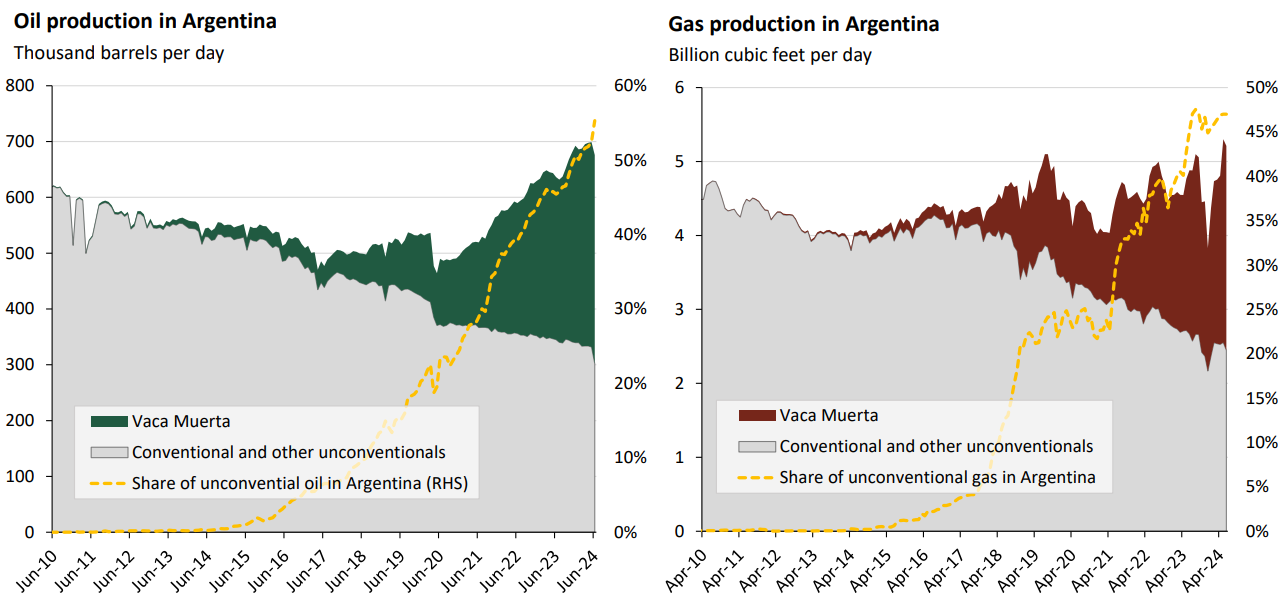
\includegraphics[width=1\linewidth]{figures/ch9/oilgasproduction.png}
    \caption{Oil and gas production in Argentina \autocite{internationaltradeadministrationArgentinaCountryCommercial2025}}
    \label{fig:oilgasprod}
\end{figure}

The numbers in \ref{fig:oilgasprod} help explain why fracking in the Neuquén basin is viewed as crucial to the development of Argentina's economy. It also becomes clear that, considering the volumes present in the reserves, even more gas and oil could still be extracted.

\section{Fracking practices}
In the 1970's, geologists became increasingly aware that large volumes of gas existed in low-permeability sandstones. However, conventional methods did not allow for economic extraction of gas from these `tight reservoirs' \autocite{tigh}. Hydraulic fracturing, or fracking, a method first tested in 1947 and applied on a large scale for the first time in the 1970's, is a modern method used to extract oil and natural gas from these low-permeability rock formations, such as shale \autocite{Fracking1012019}.

The technique begins by drilling a long vertical well. As soon as the desired rock formation is reached, drilling gradually turns horizontal and steel pipes called `casings' are inserted into the well. Small holes are perforated in the casing and then fracking fluid is pumped in at a pressure high enough to create new fractures or open existing ones in the surrounding rock. This allows previously unavailable oil or gas to flow to the surface \autocite{Fracking1012019}.

The fracking fluid contains as much as 97 percent water, but also always contains proppants. These are small, solid particles that keep the fractures in the rock formation open after the pressure from injection is removed. Sand is the most widely-used proppant in the fracking industry \autocite{Fracking1012019}.

\section{Fracking sand}
Sand used in the fracking process must have fairly specific characteristics in order to be usable for fracking. Silicon sand is mainly used for fracking. This is sand with a grain size between 0.0625 and 2.0 millimeters. The quartz grain content must be higher than 90%. 

Means of transport such as waves and currents in rivers promote the removal of finer or organic particles, thereby ensuring a higher percentage of quartz grains. This is one of the reasons why sand from the Paraná Delta is suitable for fracking.
In addition to erosion by water, the action of wind also influences the characteristics of sand. It causes changes in texture and generally makes quartz sand rounder. 

The specifications for silica sand are laid down in the international test standard ISO 13503-2:2006. The important aspects are as follows:

\begin{enumerate}
    \item  Size and distribution of the particles
    \item Shape of the particles
    \item Acid resistance 
    \item Fracture and compressive strength of the grains
    \item Clay and silt content
    \item Chemical analysis
\end{enumerate}



\section{Consequences of dry sand mining}

\section{Recommendations and mitigation strategies}